%!TEX root = ../main.tex

\section{Overview}
In this chapter various timeseries imputation and forecasting techinques are compared and results are compiled along with their implementation details. The results of the SSIM model is also described here which is an encoder decoder model the type of model normally used in machine translation techniques.

\begin{table}[h]
	\centering
	\begin{tabular}[widht=\textwidth]{|l | l |}
	\hline
	Model & MSE Score\\
	\hline
	Regression & 0.342\\
	\hline
	LSTM & 0.094\\
	\hline
	CNN & 0.0763\\
	\hline
	SSIM & 0.0944\\
	\hline
	\end{tabular}
	\caption{Comparision of time series techniques}
	\label{tab:technique-comparision-table}
\end{table}

\section{Regression}
Regression is a the core of most of the machine learning algorithm. For time series imputation regression technique can be used although it may not give the best results but it gives the fairly satisfiable results based on time taken by the algorithm to make a prediction model.

\begin{figure}[ht]
	\centering
	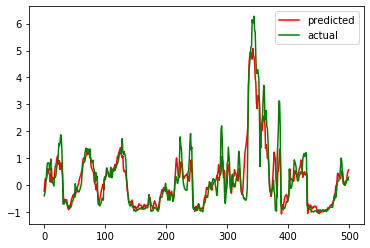
\includegraphics[width=0.8\textwidth]{images/techniques/regression.png}
	\caption{Regression PM2.5 Actual vs Predicted graph}
	\label{fig:regression-tech}
\end{figure}

 Figure \ref{fig:regression-tech} shows an actual vs predicted graph of the a regression model trained on the PM2.5 values of Beijing city. Table \ref{tab:technique-comparision-table} contains the MSE score achieved by the model.

\section{LSTM}
Long Short Term Memory(LSTM) Network is a special kind of recurrent neural network where it maintain a cell state variable which helps it to deal with the vanishing gradient problem in RNNs. It proves to be making it very feasible for time series imputation.


\begin{figure}[ht]
	\centering
	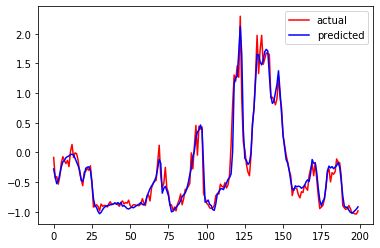
\includegraphics[width=0.8\textwidth]{images/techniques/lstm.png}
	\caption{LSTM PM2.5 Actual vs Predicted graph}
	\label{fig:lstm-tech}
\end{figure}


An LSTM model is trained on PM2.5 its MSE score is listed in table \ref{tab:technique-comparision-table}. Figure \ref{fig:lstm-tech} shows the actual vs predicted graph of the LSTM model trained on the PM2.5 values of Beijing city.

\section{CNN}
Convolutional Neural Network is very famous neural network for the field of image recognition and computer vision. It has feature of pattern detection which makes it very feasible in time series forecasting as in time series forecasting and imputation certain pattern in the data need to be exploited for making the prediction. It is generaly used with non covolutional layers in the deep learning but the main core of it is the convolutional layer which are responsible for exploiting the pattern in the data.

\begin{figure}[ht]
	\centering
	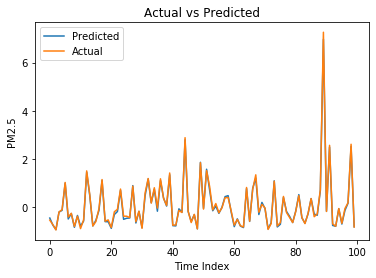
\includegraphics[width=0.8\textwidth]{images/techniques/cnn.png}
	\caption{CNN PM2.5 Actual vs Predicted graph}
	\label{fig:cnn-tech}
\end{figure}

Figure \ref{fig:cnn-tech} show the actual vs predicted graph of the CNN model trained on PM2.5 values of beijing city. Table \ref{tab:technique-comparision-table} show list the MSE score of the model.

\section{SSIM}
Sequence to Sequence Imputation Model (SSIM) is an encoder decoder model using the LSTM model as encoder attention vector is used which the encoder convert the input sequence into and another LSTM model is used as the decoder model after that a dense layer is also used for softmax values of the sequence to be generated. The working of the encoder decoder model is such that a variable length input is given to the network it converts the given input sequence to a fixed length vector known as attention vector, and the decoder convert the attention vector into the desired length sequence vector for the output.

\begin{figure}[ht]
	\centering
	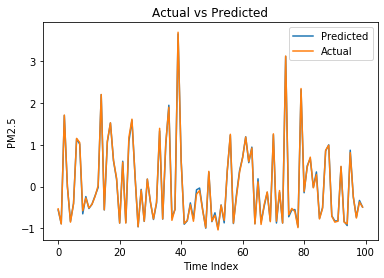
\includegraphics[width=0.8\textwidth]{images/techniques/ssim.png}
	\caption{SSIM PM2.5 Actual vs Predicted graph}
	\label{fig:ssim-tech}
\end{figure}

Figure \ref{fig:cnn-tech} show the actual vs predicted graph of the SSIM model trained on PM2.5 values of beijing city. Table \ref{tab:technique-comparision-table} show list the MSE score of the model.

\section{Summary}
In this cahpter various available machine learning and deep learning models are implemented and their mse score and actual vs predicted graphs are compared. All these model works well when they are applied on some problems where there are properly large amount of data available. In the next chapter a new approach of dealing with problem when not much data is available with hand the how deep learning models can be applied. The Transfer Learning For Time Series Imputation is applied on the two deep learning models which works well with time series problem i.e., CNN and SSIM. 